\documentclass[letterpaper,11pt]{article}

% Soporte para los acentos.
\usepackage[utf8]{inputenc}
\usepackage[T1]{fontenc}    
% Idioma español.
\usepackage[spanish,mexico, es-tabla]{babel}
% Soporte de símbolos adicionales (matemáticas)
\usepackage{multirow}
\usepackage{amsmath}
\usepackage{amssymb}
\usepackage{amsthm}
\usepackage{amsfonts}
\usepackage{mathtools}
\usepackage{latexsym}
\usepackage{enumerate}
\usepackage{ragged2e}
\usepackage{listings}
\usepackage{xcolor}
\usepackage{graphicx}
\usepackage{hyperref}
% Modificamos los márgenes del documento.
\usepackage[lmargin=1cm,rmargin=1cm,top=1.5cm,bottom=1.5cm]{geometry}

\definecolor{codegreen}{rgb}{0,0.6,0}
\definecolor{codegray}{rgb}{0.5,0.5,0.5}
\definecolor{codepurple}{rgb}{0.58,0,0.82}
\definecolor{backcolour}{rgb}{0.95,0.95,0.92}

\lstdefinestyle{mystyle}{
    backgroundcolor=\color{backcolour},   
    commentstyle=\color{codegreen},
    keywordstyle=\color{magenta},
    numberstyle=\tiny\color{codegray},
    stringstyle=\color{codepurple},
    basicstyle=\ttfamily\footnotesize,
    breakatwhitespace=false,         
    breaklines=true,                 
    captionpos=b,                    
    keepspaces=true,                 
    numbers=left,                    
    numbersep=5pt,                  
    showspaces=false,                
    showstringspaces=false,
    showtabs=false,                  
    tabsize=2
}

\lstset{style=mystyle}

\title{Facultad de Ciencias, UNAM \\ 
       Lenguajes de Programación \\ 
       Tarea 1}
\author{ \\ 
        Rubí Rojas Tania Michelle }
\date{09 de octubre de 2020}

\begin{document}
\maketitle

\begin{enumerate}
    % Ejercicio 1.
    \item Explica brevemente qué tipos de problemas puedes resolver con cada uno
    de los siguientes paradigmas y nombre un lenguaje perteneciente a cada uno.
    \begin{enumerate}
        % Ejercicio 1.a
        \item Paradigma Estructurado.
        
        \textsc{Solución:}

        % Ejercicio 1.b
        \item Paradigma Orientado a Objetos.

        \textsc{Solución:}

        % Ejercicio 1.c
        \item Paradigma Funcional.

        \textsc{Solución:}

        % Ejercicio 1.d
        \item Paradigma Lógico.

        \textsc{Solución:}
    \end{enumerate}

    % Ejercicio 2.
    \item Usando el lenguaje de programación \textsc{Prolog}, dar un ejemplo de 
    cada uno de los siguientes conceptos y justificar. No es necesario que sean 
    ejemplos demasiado elaborados.
    \begin{enumerate}
        % Ejercicio 2.a
        \item Sintaxis

        \textsc{Solución:} La sintaxis es el conjunto de reglas que debemos 
        seguir para que el compilador sea capaz de reconocer nuestro programa 
        como válido. En Prolog, todas las cláusulas de Horn (hechos y reglas) 
        deben terminar con un punto \textbf{.} 

        Por ejemplo, si queremos definir como \texttt{gatos} (hechos) a 
        \texttt{cuchis, kike} y \texttt{melisa}; y tener una regla que 
        determine las posibles parejas de gatos, entonces tendríamos un código 
        como el siguiente:
        \begin{lstlisting}[language=Prolog]
            % Hechos
            gato(cuchis).
            gato(kike).
            gato(melisa).

            % Regla
            pareja(X, Y) :- gato(X), gato(Y).
        \end{lstlisting}
        
        Donde cada una de nuestras cláusulas termina con un punto. Si llegáramos
        a omitir este último, entonces el programa no compilará porque el 
        compilador no entenderá el código y mandará un mensaje de errror al 
        programador.

        % Ejercicio 2.b
        \item Semántica

        \textsc{Solución:} La semántica es el significado que se le otorga a 
        cada una de las sentencias escritas, de acuerdo a la sintaxis definida 
        previamente en el lenguaje. En Prolog, dado el ejemplo del inciso 
        anterior, la regla \texttt{pareja} obtendrá sus valores de acuerdo a su 
        universo del discurso, el cual corresponde a los hechos sobre 
        \texttt{gatos} que hemos definido anteriormente. 

        % Ejercicio 2.c
        \item Convenciones de programación (Idioms)

        \textsc{Solución:} Son expresiones idiomáticas que son frecuentes en un 
        lenguaje. En Prolog, se tiene la convención de poner cada subobjetivo de 
        las reglas en una nueva línea. Esto mejora enormemente la legibilidad 
        del código. 
        
        Por ejemplo, 
        \begin{lstlisting}[language=Prolog]
            ord_union_all(N, Sets0, Union, Sets) :-
                A is N / 2,
                Z is N - A, 
                ord_union_all(A, Sets0, X, Sets1),
                ord_union_all(Z, Sets1, Y, Sets),
                ord_union(X, Y, Union).
        \end{lstlisting}

        Así pues, no importa qué tan cortos sean algunos subobjetivos, es mejor 
        usar una línea distinta para cada uno de ellos. 

        % Ejercicio 2.d
        \item Bibliotecas

        \textsc{Solución:} Es el conjunto de funciones previamente definidas 
        en un lenguaje, las cuales está disponibles para utilizarse por los 
        programadores. En Prolog, tenemos la biblioteca \texttt{lists}, la 
        cual nos proporciona predicados (reglas) básicos para la manipulación 
        de listas. Por ejemplo, posee la regla
        \begin{center}
            \texttt{append(?List1, ?List2, ?List1AndList2)}
        \end{center}  
        
        cuyo significado es que \texttt{List1AndList2} es la concadenación de 
        \texttt{List1} con \texttt{List2}. 

        En particular, Prolog tiene una buena documentación, aunque en la mayoría
        de los casos carece de ejemplos para mostrar cómo funciona cada una de 
        las reglas que contienen las bibliotecas.
    \end{enumerate}

    % Ejercicio 3.
    \item Dada la siguiente función, da una forma para la misma indicando el 
    tipo de entrada de los parámetros, el tipo de la salida y asígnale un nombre 
    mnemotécnico. Justifica tu respuesta. 
    \begin{verbatim}
        (define (foo n 1)
           (cond 
              [(zero? n) empty]
              [else (cons (car l) (foo (sub1 n) (cdr 1)))]))
    \end{verbatim}

    \textsc{Solución:}

    % Ejercicio 4.
    \item Para los siguientes incisos, calcular el resultado de aplicar la 
    función al parámetro recibido. Mostrar cada paso realizado hasta obtener el 
    resultado final. Da tu propia implementación para ambas funciones.
    \begin{enumerate}
        % Ejercicio 4.a
        \item \texttt{(reverse '(1 7 2 9))}
        % Ejercicio 4.b
        \item \texttt{(append '(m a n) (z a n a))}
        % Ejercicio 4.c
        \item \texttt{(reverse (append '(m a n) (z a n a)))}
    \end{enumerate} 

    \textsc{Solución:} Las implementaciones propuestas para las funciones 
    \texttt{reverse} y \texttt{append} son las siguientes 
    \begin{verbatim}
        (define (append xs ys)
          (if (empty? xs)
              ys
              (cons (car xs) (append (cdr xs) ys))))
    \end{verbatim}
    \begin{verbatim}
        (define (reverse xs)
          (if (empty? xs)
              '()
              (append (reverse (cdr xs)) (list (car xs)))))
    \end{verbatim}

    Por lo tanto, 
    \begin{enumerate}
        % Ejercicio 4.a
        \item \texttt{(reverse '(1 7 2 9))}
        \begin{align*}
            &= \texttt{(append (reverse (cdr '(1 7 2 9))) 
                               (list (car '(1 7 2 9))))} \\
            &= \texttt{(append (reverse '(7 2 9)) (list 1))} \\
            &= \texttt{(append (append (reverse (cdr '(7 2 9))) 
                                       (list (car '(7 2 9)))) '(1))} \\
            &= \texttt{(append (append (reverse '(2 9)) (list 7)) '(1))} \\
            &= \texttt{(append (append (append (reverse (cdr '(2 9)))} \\
            & \; \; \; \; \; \; \; \; \; \; \; \; \; \; \; \; \; \; \; \; \; \;  
              \; \; \; \; \; \; \; \; \; \; \; \; \; \; \; \; \; \; \; \; \; \;
              \; \; \; \; \; \;                
                                               \texttt{(list (car '(2 9)))) '(7)) '(1))} \\
            &= \texttt{(append (append (append (reverse '(9)) (list 2)) '(7)) '(1))} \\ 
            &= \texttt{(append (append (append (append (reverse (cdr '(9)))} \\ 
            & \; \; \; \; \; \; \; \; \; \; \; \; \; \; \; \; \; \; \; \; \; \;
              \; \; \; \; \; \; \; \; \; \; \; \; \; \; \; \; \; \; \; \; \; \;
              \; \; \; \; \; \; \; \; \; \; \; \; \; \; \; \; \; \; \; \; \;
                                                       \texttt{(list (car '(9)))) '(2)) '(7)) '(1))} \\
            &= \texttt{(append (append (append (append (reverse '()) (list 9)) '(2)) '(7)) '(1))} \\
            &= \texttt{(append (append (append (append '() '(9)) '(2)) '(7)) '(1))} \\
            &= \texttt{(append (append (append '(9) '(2)) '(7)) '(1))} \\
            &= \texttt{(append (append (cons (car '(9)) (append (cdr '(9)) '(2))) '(7)) '(1))} \\
            &= \texttt{(append (append (cons 9 (append '() '(2))) '(7)) '(1))} \\
            &= \texttt{(append (append (cons 9 '(2)) '(7)) '(1))} \\
            &= \texttt{(append (append '(9 2) '(7)) '(1))} \\
            &= \texttt{(append (cons (car '(9 2)) (append (cdr '(9 2)) '(7))) '(1))} \\
            &= \texttt{(append (cons 9 (append '(2) '(7))) '(1))} \\
            &= \texttt{(append (cons 9 (cons (car '(2)) (append (cdr '(2)) '(7)))) '(1))} \\ 
            &= \texttt{(append (cons 9 (cons 2 (append '() '(7)))) '(1))} \\
            &= \texttt{(append (cons 9 (cons 2 '(7))) '(1))} \\
            &= \texttt{(append (cons 9 '(2 7)) '(1))} \\
            &= \texttt{(append '(9 2 7) '(1))} \\
            &= \texttt{(cons (car '(9 2 7)) (append (cdr '(9 2 7)) '(1)))} \\
            &= \texttt{(cons 9 (append '(2 7) '(1)))} \\
            &= \texttt{(cons 9 (cons (car '(2 7)) (append (cdr '(2 7)) '(1))))} \\
            &= \texttt{(cons 9 (cons 2 (append '(7) '(1))))} \\
            &= \texttt{(cons 9 (cons 2 (cons (car '(7)) (append (cdr '(7)) '(1)))))} \\
            &= \texttt{(cons 9 (cons 2 (cons 7 (append '() '(1)))))} \\
            &= \texttt{(cons 9 (cons 2 (cons 7 '(1))))} \\
            &= \texttt{(cons 9 (cons 2 '(7 1)))} \\
            &= \texttt{(cons 9 '(2 7 1))} \\
            &= \texttt{'(9 2 7 1)}
        \end{align*}

        % Ejercicio 4.b
        \item \texttt{(append '(m a n) (z a n a))}
        \begin{align*}
            &= \texttt{(cons (car '(m a n)) (append (cdr '(m a n)) '(z a n a)))} \\
            &= \texttt{(cons m (append '(a n) '(z a n a)))} \\
            &= \texttt{(cons m (cons (car '(a n)) (append (cdr '(a n)) '(z a n a))))} \\
            &= \texttt{(cons m (cons a (append '(n) '(z a n a))))} \\
            &= \texttt{(cons m (cons a (cons (car '(n)) (append (cdr '(n)) '(z a n a)))))} \\
            &= \texttt{(cons m (cons a (cons n (append '() '(z a n a)))))} \\
            &= \texttt{(cons m (cons a (cons n '(z a n a))))} \\
            &= \texttt{(cons m (cons a '(n z a n a)))} \\
            &= \texttt{(cons m '(a n z a n a))} \\
            &= \texttt{'(m a n z a n a)}
        \end{align*}

        % Ejercicio 4.c
        \item \texttt{(reverse (append '(m a n) (z a n a)))}
        \begin{align*}
            &= \texttt{(reverse (cons (car '(m a n)) (append (cdr '(m a n)) '(z a n a))))} \\
            &= \texttt{(reverse (cons m (append '(a n) '(z a n a))))} \\
            &= \texttt{(reverse (cons m (cons (car '(a n)) (append (cdr '(a n)) '(z a n a)))))} \\
            &= \texttt{(reverse (cons m (cons a (append '(n) '(z a n a)))))} \\
            &= \texttt{(reverse (cons m (cons a (cons (car '(n)) (append (cdr '(n)) '(z a n a))))))} \\
            &= \texttt{(reverse (cons m (cons a (cons n (append '() '(z a n a))))))} \\
            &= \texttt{(reverse (cons m (cons a (cons n '(z a n a)))))} \\
            &= \texttt{(reverse (cons m (cons a '(n z a n a))))} \\
            &= \texttt{(reverse (cons m '(a n z a n a)))} \\
            &= \texttt{(reverse '(m a n z a n a))} \\
            &= \texttt{(append (reverse (cdr '(m a n z a n a))) (list (car '(m a n z a n a))))} \\
            &= \texttt{(append (reverse '(a n z a n a)) (list m))} \\
            &= \texttt{(append (append (reverse (cdr '(a n z a n a))) (list (car '(a n z a n a)))) '(m))} \\
            &= \texttt{(append (append (reverse '(n z a n a)) (list a)) '(m))} \\
            &= \texttt{(append (append (append (reverse (cdr '(n z a n a))) (list (car '(n z a n a))))} \\
            & \; \; \; \; \; \; \; \; \; \; \; \; \; \; \; \; \; \; \; \; \; \; \; 
              \; \; \; \; \; \; \; \; \; \; \; \; 
                                       \texttt{'(a)) '(m))} \\
            &= \texttt{(append (append (append (reverse '(z a n a)) (list n)) '(a)) '(m))} \\
            &= \texttt{(append (append (append (append (reverse (cdr '(z a n a))) (list (car '(z a n a))))} \\
            & \; \; \; \; \; \; \; \; \; \; \; \; \; \; \; \; \; \; \; \; \; \; \;
              \; \; \; \; \; \; \; \; \; \; \; \; \; \; \; \; \; \; \; \; \; \; \;
              \; \; \; \;  
                                               \texttt{'(n)) '(a)) '(m))} \\
            &= \texttt{(append (append (append (append (reverse '(a n a)) (list z)) '(n)) '(a)) '(m))} \\
            &= \texttt{(append (append (append (append (append (reverse (cdr '(a n a))) (list (car '(a n a))))} \\
            & \; \; \; \; \; \; \; \; \; \; \; \; \; \; \; \; \; \; \; \; \; \; \;
              \; \; \; \; \; \; \; \; \; \; \; \; \; \; \; \; \; \; \; \; \; \; \;
              \; \; \; \; \; \; \; \; \; \; \; \; \; \; \; \; \; \; \; 
                                                       \texttt{'(z)) '(n)) '(a)) '(m))} \\
            &= \texttt{(append (append (append (append (append (reverse '(n a)) (list a)) '(z)) '(n))} \\ 
            & \; \; \; \; \; \; \; \; \; \; \; \; \; \; \; \; \; \; \; \; \; \; \; 
              \; \; \; \; \; \; \; \; \; \; \; \; 
                                       \texttt{'(a)) '(m))} \\ 
            &= \texttt{(append (append (append (append (append (append (reverse (cdr '(n a)))} \\ 
            & \; \; \; \; \; \; \; \; \; \; \; \; \; \; \; \; \; \; \; \; \; \; \;
              \; \; \; \; \; \; \; \; \; \; \; \; \; \; \; \; \; \; \; \; \; \; \;
              \; \; \; \; \; \; \; \; \; \; \; \; \; \; \; \; \; \; \; \; \; \; \;
              \; \; \; \; \; \; \; \; \; \; \; \; \; \; \; \; \; \; \; \; \; \; \;
              \; \;
                                                                       \texttt{(list (car '(n a))))} \\
            & \; \; \; \; \; \; \; \; \; \; \; \; \; \; \; \; \; \; \; \; \; \; \;
              \; \; \; \; \; \; \; \; \; \; \; \; \; \; \; \; \; \; \; \; \; \; \;
              \; \; \; \; \; \; \; \; \; \; \; \; \; \; \; \; \; \; \; \; \; \; \;
              \; \; \; \; \; \; \; \; \; \; \;
                                                               \texttt{'(a)) '(z)) '(n)) '(a)) '(m))} \\
            &= \texttt{(append (append (append (append (append (append (reverse '(a)) (list n))} \\
            & \; \; \; \; \; \; \; \; \; \; \; \; \; \; \; \; \; \; \; \; \; \; \;
              \; \; \; \; \; \; \; \; \; \; \; \; \; \; \; \; \; \; \; \; \; \; \;
              \; \; \; \; \; \; \; \; \; \; \; \; \; \; \; \; \; \; \; \; \; \; \;
              \; \; \; \; \; \; \; \; \; \; \; \texttt{'(a)) '(z)) '(n)) '(a)) '(m))} \\
            &= \texttt{(append (append (append (append (append (append (append (reverse (cdr '(a)))} \\ 
            & \; \; \; \; \; \; \; \; \; \; \; \; \; \; \; \; \; \; \; \; \; \; \;
              \; \; \; \; \; \; \; \; \; \; \; \; \; \; \; \; \; \; \; \; \; \; \;
              \; \; \; \; \; \; \; \; \; \; \; \; \; \; \; \; \; \; \; \; \; \; \;
              \; \; \; \; \; \; \; \; \; \; \; \; \; \; \; \; \; \; \; \; \; \; \;
              \; \; \; \; \; \; \; \; \; \; \; \; \; \; \; \; \; 
                                                                               \texttt{(list (car '(a))))} \\ 
            & \; \; \; \; \; \; \; \; \; \; \; \; \; \; \; \; \; \; \; \; \; \; \;
              \; \; \; \; \; \; \; \; \; \; \; \; \; \; \; \; \; \; \; \; \; \; \;
              \; \; \; \; \; \; \; \; \; \; \; \; \; \; \; \; \; \; \; \; \; \; \;
              \; \; \; \; \; \; \; \; \; \; \; \; \; \; \; \; \; \; \; \; \; \; \;
              \; \; 
                                                                       \texttt{'(n)) '(a)) '(z)) '(n)) '(a)) '(m))} \\
            &= \texttt{(append (append (append (append (append (append (append (reverse '()) (list a))} \\
            & \; \; \; \; \; \; \; \; \; \; \; \; \; \; \; \; \; \; \; \; \; \; \;
              \; \; \; \; \; \; \; \; \; \; \; \; \; \; \; \; \; \; \; \; \; \; \;
              \; \; \; \; \; \; \; \; \; \; \; \; \; \; \; \; \; \; \; \; \; \; \;
              \; \; \; \; \; \; \; \; \; \; \; \; \; \; \; \; \; \; \; \; \; \; \;
              \; \; 
                                                                       \texttt{'(n)) '(a)) '(z)) '(n)) '(a)) '(m))} \\
            &= \texttt{(append (append (append (append (append (append (append '() '(a))} \\
            & \; \; \; \; \; \; \; \; \; \; \; \; \; \; \; \; \; \; \; \; \; \; \;
              \; \; \; \; \; \; \; \; \; \; \; \; \; \; \; \; \; \; \; \; \; \; \;
              \; \; \; \; \; \; \; \; \; \; \; \; \; \; \; \; \; \; \; \; \; \; \;
              \; \; \; \; \; \; \; \; \; \; \; \; \; \; \; \; \; \; \; \; \; \; \;
              \; \; 
                                                                       \texttt{'(n)) '(a)) '(z)) '(n)) '(a)) '(m))} \\
            &= \texttt{(append (append (append (append (append (append '(a) '(n)) '(a)) '(z)) '(n)) '(a)) '(m))} \\
        \end{align*}
        \begin{align*}
            &= \texttt{(append (append (append (append (append (cons (car '(a)) (append (cdr '(a)) '(n)))} \\ 
            & \; \; \; \; \; \; \; \; \; \; \; \; \; \; \; \; \; \; \; \; \; \; \;
              \; \; \; \; \; \; \; \; \; \; \; \; \; \; \; \; \; \; \; \; \; \; \;
              \; \; \; \; \; \; \; \; \; \; \; \; \; \; \; \; \; \; \; \; \; \; \; 
              \; \; \; \; \; \; \; \; \; \; 
                                                       \texttt{'(a)) '(z)) '(n)) '(a)) '(m))} \\
            &= \texttt{(append (append (append (append (append (cons a (append '() '(n)))} \\ 
            & \; \; \; \; \; \; \; \; \; \; \; \; \; \; \; \; \; \; \; \; \; \; \;
              \; \; \; \; \; \; \; \; \; \; \; \; \; \; \; \; \; \; \; \; \; \; \;
              \; \; \; \; \; \; \; \; \; \; \; \; \; \; \; \; \; \; \; \; \; \; \; 
              \; \; \; \; \; \; \; \; \; \; 
                                                       \texttt{'(a)) '(z)) '(n)) '(a)) '(m))} \\
            &= \texttt{(append (append (append (append (append (cons a '(n)) '(a)) '(z)) '(n)) '(a)) '(m))} \\
            &= \texttt{(append (append (append (append (append '(a n) '(a)) '(z)) '(n)) '(a)) '(m))} \\ 
            &= \texttt{(append (append (append (append (cons (car '(a n)) (append (cdr '(a n)) '(a)))} \\
            & \; \; \; \; \; \; \; \; \; \; \; \; \; \; \; \; \; \; \; \; \; \; \;
              \; \; \; \; \; \; \; \; \; \; \; \; \; \; \; \; \; \; \; \; \; \; \;
              \; \; \; \; \; \; \; \; \; \; \; \; \; \; \; \; \; \;
                                                       \texttt{'(z)) '(n)) '(a)) '(m))} \\
            &= \texttt{(append (append (append (append (cons a (append '(n) '(a))) '(z)) '(n)) '(a)) '(m))} \\
            &= \texttt{(append (append (append (append (cons a (cons (car '(n)) (append (cdr '(n)) '(a))))} \\
            & \; \; \; \; \; \; \; \; \; \; \; \; \; \; \; \; \; \; \; \; \; \; \;
            \; \; \; \; \; \; \; \; \; \; \; \; \; \; \; \; \; \; \; \; \; \; \;
            \; \; \; \; \; \; \; \; \; \; \; \; \; \; \; \; \; \;
                                                       \texttt{'(z)) '(n)) '(a)) '(m))} \\
            &= \texttt{(append (append (append (append (cons a (cons n (append '() '(a))))} \\ 
            & \; \; \; \; \; \; \; \; \; \; \; \; \; \; \; \; \; \; \; \; \; \; \;
            \; \; \; \; \; \; \; \; \; \; \; \; \; \; \; \; \; \; \; \; \; \; \;
            \; \; \; \; \; \; \; \; \; \; \; \; \; \; \; \; \; \;
                                                       \texttt{'(z)) '(n)) '(a)) '(m))} \\
            &= \texttt{(append (append (append (append (cons a (cons n '(a))) '(z)) '(n)) '(a)) '(m))} \\
            &= \texttt{(append (append (append (append (cons a '(n a)) '(z)) '(n)) '(a)) '(m))} \\
            &= \texttt{(append (append (append (append '(a n a) '(z)) '(n)) '(a)) '(m))} \\
            &= \texttt{(append (append (append (cons (car '(a n a)) (append (cdr '(a n a)) '(z)))} \\
            & \; \; \; \; \; \; \; \; \; \; \; \; \; \; \; \; \; \; \; \; \; \; \;
            \; \; \; \; \; \; \; \; \; \; \; \; \; \; \; \; \; \; \; \; \; \; \;
            \; \; \; 
                                               \texttt{'(n)) '(a)) '(m))} \\
            &= \texttt{(append (append (append (cons a (append '(n a) '(z))) '(n)) '(a)) '(m))} \\
            &= \texttt{(append (append (append (cons a (cons (car '(n a)) (append (cdr '(n a)) '(z))))} \\
            & \; \; \; \; \; \; \; \; \; \; \; \; \; \; \; \; \; \; \; \; \; \; \;
            \; \; \; \; \; \; \; \; \; \; \; \; \; \; \; \; \; \; \; \; \; \; \;
            \; \; \; 
                                               \texttt{'(n)) '(a)) '(m))} \\
            &= \texttt{(append (append (append (cons a (cons n (append '(a) '(z)))) '(n)) '(a)) '(m))} \\
            &= \texttt{(append (append (append (cons a (cons n (cons (car '(a)) (append (cdr '(a)) '(z)))))} \\
            & \; \; \; \; \; \; \; \; \; \; \; \; \; \; \; \; \; \; \; \; \; \; \;
            \; \; \; \; \; \; \; \; \; \; \; \; \; \; \; \; \; \; \; \; \; \; \;
            \; \; \; 
                                               \texttt{'(n)) '(a)) '(m))} \\
            &= \texttt{(append (append (append (cons a (cons n (cons a (append '() '(z)))))} \\
            & \; \; \; \; \; \; \; \; \; \; \; \; \; \; \; \; \; \; \; \; \; \; \;
            \; \; \; \; \; \; \; \; \; \; \; \; \; \; \; \; \; \; \; \; \; \; \;
            \; \; \; 
                                               \texttt{'(n)) '(a)) '(m))} \\
            &= \texttt{(append (append (append (cons a (cons n (cons a '(z)))) '(n)) '(a)) '(m))} \\
            &= \texttt{(append (append (append (cons a (cons n '(a z))) '(n)) '(a)) '(m))} \\
            &= \texttt{(append (append (append (cons a '(n a z)) '(n)) '(a)) '(m))} \\
            &= \texttt{(append (append (append '(a n a z) '(n)) '(a)) '(m))} \\
            &= \texttt{(append (append (cons (car '(a n a z)) (append (cdr '(a n a z)) '(n))) '(a)) '(m))} \\
            &= \texttt{(append (append (cons a (append '(n a z) '(n))) '(a)) '(m))} \\
            &= \texttt{(append (append (cons a (cons (car '(n a z)) (append (cdr '(n a z)) '(n))))} \\
            & \; \; \; \; \; \; \; \; \; \; \; \; \; \; \; \; \; \; \; \; \; \; \;
            \; \; \; \; \; \; \; \; \; \; \; 
                                       \texttt{'(a)) '(m))} \\
            &= \texttt{(append (append (cons a (cons n (append '(a z) '(n)))) '(a)) '(m))} \\
            &= \texttt{(append (append (cons a (cons n (cons (car '(a z)) (append (cdr '(a z)) '(n)))))} \\
            & \; \; \; \; \; \; \; \; \; \; \; \; \; \; \; \; \; \; \; \; \; \; \;
            \; \; \; \; \; \; \; \; \; \; \; 
                                       \texttt{'(a)) '(m))} \\
            &= \texttt{(append (append (cons a (cons n (cons a (append '(z) '(n))))) '(a)) '(m))} \\
            &= \texttt{(append (append (cons a (cons n (cons a (cons (car '(z)) (append (cdr '(z)) '(n))))))} \\
            & \; \; \; \; \; \; \; \; \; \; \; \; \; \; \; \; \; \; \; \; \; \; \;
            \; \; \; \; \; \; \; \; \; \; \; 
                                       \texttt{'(a)) '(m))} \\
            &= \texttt{(append (append (cons a (cons n (cons a (cons z (append '() '(n)))))) '(a)) '(m))} \\
            &= \texttt{(append (append (cons a (cons n (cons a (cons z '(n))))) '(a)) '(m))} \\
            &= \texttt{(append (append (cons a (cons n (cons a '(z n)))) '(a)) '(m))} \\
            &= \texttt{(append (append (cons a (cons n '(a z n))) '(a)) '(m))} \\
        \end{align*}
        \begin{align*}
            &= \texttt{(append (append (cons a '(n a z n)) '(a)) '(m))} \\
            &= \texttt{(append (append '(a n a z n) '(a)) '(m))} \\
            &= \texttt{(append (cons (car '(a n a z n)) (append (cdr '(a n a z n)) '(a))) '(m))} \\
            &= \texttt{(append (cons a (append '(n a z n) '(a))) '(m))} \\
            &= \texttt{(append (cons a (cons (car '(n a z n)) (append (cdr '(n a z n)) '(a)))) '(m))} \\
            &= \texttt{(append (cons a (cons n (append '(a z n) '(a)))) '(m))} \\
            &= \texttt{(append (cons a (cons n (cons (car '(a z n)) (append (cdr '(a z n)) '(a))))) '(m))} \\
            &= \texttt{(append (cons a (cons n (cons a (append '(z n) '(a))))) '(m))} \\
            &= \texttt{(append (cons a (cons n (cons a (cons (car '(z n)) (append (cdr '(z n)) '(a)))))) '(m))} \\
            &= \texttt{(append (cons a (cons n (cons a (cons z (append '(n) '(a)))))) '(m))} \\
            &= \texttt{(append (cons a (cons n (cons a (cons z (cons (car '(n)) (append (cdr '(n)) '(a))))))) (m))} \\
            &= \texttt{(append (cons a (cons n (cons a (cons z (cons n (append '() '(a))))))) '(m))} \\
            &= \texttt{(append (cons a (cons n (cons a (cons z (cons n '(a)))))) '(m))} \\
            &= \texttt{(append (cons a (cons n (cons a (cons z '(n a))))) '(m))} \\
            &= \texttt{(append (cons a (cons n (cons a '(z n a)))) '(m))} \\
            &= \texttt{(append (cons a (cons n '(a z n a))) '(m))} \\
            &= \texttt{(append (cons a '(n a z n a)) '(m))} \\
            &= \texttt{(append '(a n a z n a) '(m))} \\
            &= \texttt{(cons (car '(a n a z n a)) (append (cdr '(a n a z n a)) '(m)))} \\
            &= \texttt{(cons a (append '(n a z n a) '(m)))} \\
            &= \texttt{(cons a (cons (car '(n a z n a)) (append (cdr '(n a z n a)) '(m))))} \\
            &= \texttt{(cons a (cons n (append '(a z n a) '(m))))} \\
            &= \texttt{(cons a (cons n (cons (car '(a z n a)) (append (cdr '(a z n a)) '(m)))))} \\
            &= \texttt{(cons a (cons n (cons a (append '(z n a) '(m)))))} \\
            &= \texttt{(cons a (cons n (cons a (cons (car '(z n a)) (append (cdr '(z n a)) '(m))))))} \\
            &= \texttt{(cons a (cons n (cons a (cons z (append '(n a) '(m))))))} \\
            &= \texttt{(cons a (cons n (cons a (cons z (cons (car '(n a)) (append (cdr '(n a)) '(m)))))))} \\
            &= \texttt{(cons a (cons n (cons a (cons z (cons n (append '(a) '(m)))))))} \\
            &= \texttt{(cons a (cons n (cons a (cons z (cons n (cons (car '(a)) (append (cdr '(a)) '(m))))))))} \\
            &= \texttt{(cons a (cons n (cons a (cons z (cons n (cons a (append '() '(m))))))))} \\
            &= \texttt{(cons a (cons n (cons a (cons z (cons n (cons a '(m)))))))} \\
            &= \texttt{(cons a (cons n (cons a (cons z (cons n '(a m))))))} \\
            &= \texttt{(cons a (cons n (cons a (cons z '(n a m)))))} \\
            &= \texttt{(cons a (cons n (cons a '(z n a m))))} \\
            &= \texttt{(cons a (cons n '(a z n a m)))} \\
            &= \texttt{(cons a '(n a z n a m))} \\
            &= \texttt{'(a n a z n a m)}
        \end{align*}
    \end{enumerate}

    % Ejercicio 5.
    \item Da una tabla donde expliques las principales diferencias entre un 
    compilador y un intérprete.

    \textsc{Solución:}

    % Ejercicio 6.
    \item Dibuja un mapa mental que muestre las fases de generación de código
    ejecutable, sus principales características y elementos involucrados.

    \textsc{Solución:} Las fases de generación de código ejecutable son aquellas 
    que analzan, modifican y optimizan el código para que la computadora lo 
    pueda entender. El siguiente mapa mental describe el órden de estas fases.
    \begin{figure}[ht]
        \centering
        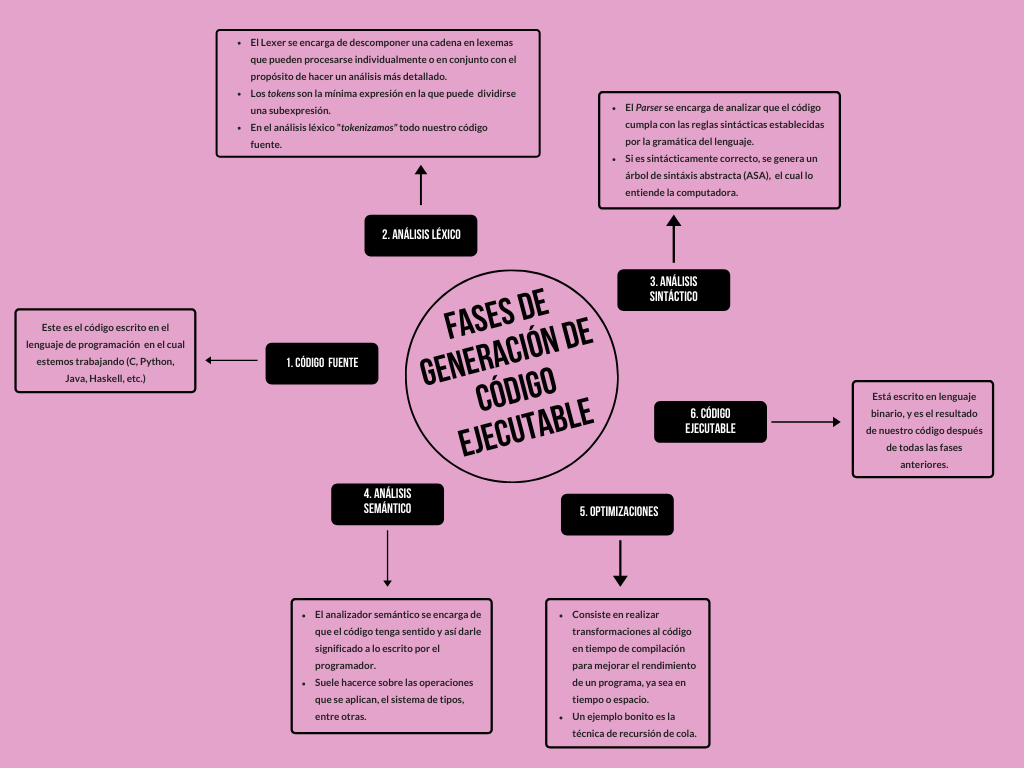
\includegraphics[width=0.9\textwidth]{./imagenes/Fases de generación de código.png}
    \end{figure}

    % Ejercicio 7.
    \item Dadas las siguientes expresiones de AE en sintaxis concreta, da su 
    respectiva representación en sintaxis abstracta por medio de los Árboles 
    de Sintaxos Abstracta correspondientes. En caso de no poder generar el
    árbol, justificar. 
    \begin{enumerate}
        \item \texttt{\{+ 18 \{- 15 \{+ 40 5\}\}\}}
        
        \textsc{Solución:} Tenemos que 
        \begin{align*}
            \texttt{(parse '\{+ 18 \{- 15 \{+ 40 5\}\}\})}
            &= \texttt{(add (parse '18) (parse '\{- 15 \{+ 40 5\}\}))} \\
            &= \texttt{(add (num 18) (sub (parse '15) (parse '\{+ 40 5\})))} \\
            &= \texttt{(add (num 18) (sub (num 15) (add (parse '40) (parse '5))))} \\
            &= \texttt{(add (num 18) (sub (num 15) (add (num 40) (num 5))))}
        \end{align*}

        Por lo tanto, su representación en sintaxis abstracta es 
        \begin{center}
            \texttt{(add (num 18) (sub (num 15) (add (num 40) (num 5))))}
        \end{center}

        \item \texttt{\{+ \{- 15 \{+ 40\}\}\}}

        \textsc{Solución:} No es posible generar el árbol ya que el operador 
        \texttt{+} es binario, y en las dos ocasiones en que es utiliza, falta 
        alguna expresión de AE en el lado izquierdo. Así, al momento de
        querer aplicar el \texttt{parser}, este hecho hará que falle nuestra 
        función y no podamos generar el árbol. 
    \end{enumerate}
\end{enumerate}

\begin{thebibliography}{10}
    \bibitem{1}
    Coding Guidelines for Prolog \\ 
    \url{https://www.cs.unipr.it/~bagnara/Papers/PDF/TPLP12.pdf}

    \bibitem{2} 
    A.21 library(lists): List Manipulation \\
    \url{https://www.swi-prolog.org/pldoc/man?section=lists}

    \bibitem{3}
    Sintaxis de Prolog \\
    \url{http://gpd.sip.ucm.es/jaime/pl/prolog.pdf}

    \bibitem{4}
    Sintáxis y semántica de Prolog \\
    \url{https://es.qaz.wiki/wiki/Prolog_syntax_and_semantics#Semantics}
\end{thebibliography}

\end{document}
